\glspl{MSR} are one of six advanced reactor designs shortlisted by
the Generation IV Forum in 2001 for promising significant advances in safety,
sustainability, efficiency, and cost over existing designs. This
has attracted significant attention and resources towards
\gls{MSR} research, most noticeable by the number of start-up companies that
have emerged in recent years touting various \gls{MSR} designs. This chapter
provides a brief history of \glspl{MSR}, followed by the distinctive features
that earned the concept the label of being a Generation IV reactor. Lastly,
this chapter presents the reference specifications of the \gls{MSFR} concept
studied in this work.

\section{History}

The first \gls{MSR}, named the \gls{ARE}, dates back to the 1940s
as part of the US Aircraft Nuclear Propulsion program
\cite{rosenthal_molten-salt_1970}. Researchers recommended the molten fluoride
salts in particular for high uranium solubility, chemical stability, low vapor
pressure even at high temperatures, decent heat transfer properties,
resistance against radiation damage, and reduced corrosive effects on some
common structural material \cite{rosenthal_molten-salt_1970}. They
subsequently built the 2.5 MW$_{\text{th}}$ ARE reactor at \gls{ORNL}, where
it achieved criticality on November 1954 and generated 100 MWh over nine days.
The fuel consisted of enriched uranium in a molten salt mixture of NaF,
ZrF$_4$, and UF$_4$, and the reactor used blocks of BeO for neutron
moderation. The aircraft program
ultimately never came to fruition as the development of intercontinental
ballistic missiles effectively eliminated the need for long-range
nuclear-powered bomber aircraft.

However, the successful demonstration of the \gls{ARE} spurred further
research into adapting \glspl{MSR} for civilian power generation
\cite{rosenthal_molten-salt_1970}. One key finding from the
research was that the thorium fuel cycle had a better breeding ratio than the
$^{238}$U-to-$^{239}$Pu fuel cycle in thermal-spectrum reactors.
Ultimately, these efforts culminated in the design, construction, and
successful operation of the \gls{MSRE}, a graphite-moderated thermal
\gls{MSR}. The \gls{MSRE} had a
graphite-moderated design with a LiF-BeF$_2$-ZrF$_4$-UF$_4$ fuel salt mixture,
initially rated at 10 MW$_{\text{th}}$ but later restricted to 8
MW$_{\text{th}}$ due to a miscalculation of heat transfer capabilities
\cite{haubenreich_experience_1970}. In January 1969, the \gls{MSRE} became the
first reactor to run on $^{233}$U fuel.

Building on their experience with the \gls{MSRE}, \gls{ORNL} proposed a
new program for the construction and operation of a demonstration reactor
based on the Molten Salt Breeder Reactor (MSBR) concept that they had
developed \cite{macpherson_molten_1985}. The \gls{MSBR} is a thermal-spectrum,
single fluid reactor with fertile $^{232}$Th isotopes mixed directly into the
FLiBe molten salt for $^{233}$U breeding \cite{gehin_liquid_2016}. Like the
\gls{MSRE}, the \gls{MSBR} relies on continuous online reprocessing to add
fertile material and remove fission product neutron poisons. Researchers
estimated the doubling time (the minimum amount of time required to produce
enough fissile material to start up another \gls{MSBR}) to be
approximately 22 years. However, \gls{ORNL} failed to secure funding for the
new program in their two attempts in 1972 and 1974. Nevertheless, from a
technical perspective, two independent
technology evaluation and design studies of the \gls{MSR} had reported
favorably on the promise of the system \cite{macpherson_molten_1985}.

In spite of this setback, research into \glspl{MSR} continued through the late
1970s. In 1980, \gls{ORNL} published a report describing a new \gls{MSR}
concept, called the \gls{DMSR} \cite{gehin_liquid_2016} with denatured
$^{235}$U fuel (i.e. low-enriched uranium). The \gls{ORNL} researchers
developed this design in response to the fuel reprocessing restrictions
introduced by President Ford in 1976. The \gls{DMSR} would operate as a
once-through
converter system without fuel reprocessing. While the fuel largely consists of
19.75 \% \gls{HALEU}, the initial core loading includes thorium to
boost its conversion ratio throughout its lifetime. It has a continuous
online feed consisting of \gls{HALEU} to maintain criticality, and denatured
$^{235}$U to keep uranium enrichment levels below nuclear non-proliferation
policy thresholds. The design also includes a gas sparging system for removing
gaseous fission products, while noble metals plate out onto the walls of
the coolant loop. The older \gls{MSBR} design had a significant drawback; the
extensive neutron damage in the graphite moderator necessitated frequent
replacement (every four years) throughout its operational lifetime. The
\gls{DMSR} avoids this issue by having a lower power density while maintaining
the overall power output of 2250 MW$_{\text{th}}$. As a result, researchers
projected that the graphite moderator would last for the entirety of the
\gls{DMSR}'s design lifetime.

There was a concurrent program at the UK Atomic Energy Authority for the
development of a 2500 MW$_{\text{e}}$ lead-cooled
\gls{MCFR} concept \cite{smith_assessment_1974}. It is a dual fluid system,
with separate loops for the fuel salt and the blanket salt. The blanket is a
1 m-wide tank surrounding the core. The absence of moderators and the choice
of chloride over fluoride salt resulted in a relatively hard neutron spectrum
which favors $^{239}$Pu breeding over the thorium cycle. The UK researchers
performed some experiments to study molten salt chemistry but there were no
reactor prototypes. The UK program eventually shut down just like its
US counterpart partly due to the successful demonstration of the Prototype
Fast Reactor which had achieved criticality in 1974.

Following a lull lasting through the late 20th century, \gls{MSR} research
picked up pace due to renewed interest initiated by the Generation IV Forum in
2001. Today, there are numerous \gls{MSR} concepts under active development
led by various national and commercial bodies.

\section{Features}

As mentioned in Chapter \ref{chap:intro}, the most significant difference
between \glspl{MSR} and other reactor concepts is the liquid fuel in
\glspl{MSR}; fissile and/or fertile material is dissolved in high temperature,
commonly eutectic mixtures of molten salts. Molten salt-cooled, solid-fuel
reactors also exist but this thesis will focus on liquid-fuel reactors.
The primary coolant loop containing the fuel salt
transfers heat through a heat exchanger to the clean, intermediate
loop. The liquid fuel form allows for continuous online fuel reprocessing,
and the removal of gaseous fission products via a gas sparging system.

The various \gls{MSR} designs under development today illustrate the
flexibility of this reactor concept. Graphite-moderated thermal-spectrum
\glspl{MSR} are typically straightforward \gls{LEU} burners or
$^{232}$Th/$^{233}$U iso-breeders/breeders, while epithermal- and
fast-spectrum \glspl{MSR} can operate as \gls{TRU} fuel burners or
$^{238}$U/$^{239}$Pu breeders. Breeder designs can be further categorized into
one- or two-fluid designs. Two-fluid designs feature separate blanket molten
salt mixtures that contain higher proportions of fertile material than the
fuel salt mixture. Examples of one-fluid designs include the Integral Molten
Salt Reactor from Terrestrial Energy \cite{leblanc_integral_2015} and the
\gls{MSR} design from Transatomic Power
\cite{transatomic_power_corporation_technical_2016} while two-fluid designs
include the \gls{MSFR} \cite{serp_molten_2014} and \gls{MOSART}
\cite{ignatiev_molten_2014}.

\subsection{Safety}

\glspl{MSR} rely on natural physical phenomena for passive safety such as the
strong negative temperature reactivity feedback of the fuel salt due to
greater temperature-induced expansion in liquid fuel than solid
fuel. Combined with the Doppler broadening of resonance capture cross sections
present in both fuel forms, there would be a smaller temperature
increase following an unprotected reactivity insertion. The overall
temperature reactivity coefficient varies widely among \gls{MSR}
designs due to other structures, such as moderators and reflectors, present in
the core. In particular, graphite moderators tend to have slightly positive
temperature reactivity coefficients. \gls{MSBR} concept has this issue, but
the total temperature reactivity coefficient is still relatively large and
negative \cite{rykhlevskii_modeling_2019}. The negative temperature reactivity
feedback provides a large degree of control and stability as it is always
present in an \gls{MSR} regardless of the operating conditions.

Continuous online fuel reprocessing allows operators to maintain low excess
reactivity inventories in the core as additional fuel can be added on an ad
hoc basis. Reprocessing and gas sparging systems help reduce fissile
requirements by continuously removing neutron poisons. These factors, in
addition to the strong negative temperature
reactivity coefficient, diminish the likelihood and severity of unprotected
criticality accidents in \glspl{MSR} \cite{elsheikh_safety_2013}. In the
unlikely situation in which an \gls{MSR} encounters a severe runaway reaction,
\glspl{MSR} rely on another passive safety feature: freeze plugs. Various
freeze plugs designs exist for different \glspl{MSR}. The freeze plug
in the \gls{MSFR} concept is a plug of solidified salt at the bottom of the
core actively cooled by fans or other cooling systems to keep its temperature
just below the freezing point of the salt \cite{aji_experimental_2020}. In
general, when temperatures in the core exceed a certain threshold during a
dangerous transient, the freeze plug melts and the molten salt in the core
drains into a containment tank designed to keep the salt in a subcritical
configuration. This is especially easy to achieve in thermal-spectrum
\glspl{MSR} as the absence of moderators in the containment tank would
automatically drive the multiplication factor down below unity
\cite{elsheikh_safety_2013}.

During pump failure accidents, natural circulation can passively sustain
enough heat transfer to remove decay heat and prevent catastrophic structural
failure. If natural circulation proves insufficient, the aforementioned freeze
plug can drain the salt out of the core. Decay heat in \glspl{MSR} with online
reprocessing is typically lower than that in \glspl{LWR} due to the
continuous removal of fission products. For example, the decay heat in an
\gls{MSFR} after reaching equilibrium salt composition is approximately
3.5\% of full reactor power compared to 6\% in \glspl{LWR}
\cite{brovchenko_design-related_2013}.

\glspl{MSR} also typically have large margin-to-boiling under nominal
operating conditions so that fuel salt boiling does not occur
\cite{elsheikh_safety_2013}. Furthermore, the reactor vessel is consequently
subject to much lower stresses as \glspl{MSR} operate at near-atmospheric
pressure levels. Thus, the probability of pipe ruptures due to high pressure
is low.

However, there are also some safety disadvantages associated with \glspl{MSR}.
Firstly, \glspl{MSR} have smaller fractions of delayed neutron precursors in
the active core region as some of them decay in the external loop regions.
This complicates reactor control and may result in faster transients due to
the decrease in average neutron lifetime. Secondly, hot molten salts are
generally corrosive and the corrosion mechanism is different from conventional
corrosion induced by water and other common agents \cite{yoshioka_7_2017}. The
intense gamma and neutron radiation in the core may also accelerate corrosion
in the structural components. Lastly, overcooling in pipes and heat exchangers
may pose operational challenges as the salt can freeze and restrict flow,
thereby causing a loss of flow accident \cite{ho_molten_2013}.

\subsection{Other Features}

\glspl{MSR} have several positive sustainability features.
\glspl{MSR} have good neutron economy due to the continuous removal of
neutron poisons by the online reprocessing and gas sparging systems
\cite{kamei_recent_2012}. Both
$^{232}$Th/$^{233}$U and $^{238}$U/$^{239}$Pu fuel cycles are viable
candidates for breeding in \glspl{MSR}, with the former being more suited for
thermal reactors and the latter being more suited for fast reactors.

The $^{232}$Th/$^{233}$U fuel cycle produces significantly less \gls{TRU}
waste than the other cycles due to the smaller atomic masses of $^{232}$Th and
$^{233}$U. This reduces the overall radiotoxicity and long-term decay heat
associated with long-lived plutonium and \gls{MA} isotopes. The combination
of \gls{TRU} fuel and $^{232}$Th feed in fast spectrum \glspl{MSR} would help
reduce overall levels of \gls{TRU} waste going into long-term storage in
nuclear waste repositories \cite{merle-lucotte_launching_2011}.

Nuclear non-proliferation concerns in thorium-fueled \glspl{MSR} involve the
separation of the intermediate $^{233}$Pa
isotope from the fuel salt. $^{233}$Pa decays into $^{233}$U with a half-life
of approximately 27 days and the $^{233}$U produced is equivalent in potency
to $^{239}$Pu for nuclear weapons production \cite{grape_10_2017}. The highly
radioactive $^{232}$U
by-product provides some level of proliferation resistance but nuclear
proliferators can sidestep this complication by
separating the $^{232}$U away from the combined $^{232}$Pa/$^{233}$Pa stream
after most of the $^{232}$Pa has decayed into $^{232}$U at a short half-life
of 1.31 days \cite{grape_10_2017}. Safeguards by design and close monitoring
of \glspl{MSR} are therefore essential to avoiding spent nuclear fuel
diversion.

Economic analyses of \glspl{MSR} are preliminary at the current
stage of \gls{MSR} development. Qualitatively, many technical factors favor
\glspl{MSR} over \gls{LWR}. Some of these factors include: smaller reactor
core size due to low operating pressures, higher thermal efficiency and
cheaper air-cooling systems due to high operating temperatures, reduction in
fuel fabrication costs, and shorter reactor shutdown periods due to online
refueling \cite{dolan_1_2017}. Moir \cite{moir_recommendations_2008}
published data from \gls{ORNL} reports on the estimated electricity costs for
a 1000 MWe \gls{MSR} with 20\% enriched $^{235}$U fuel and no reprocessing
throughout the reactor's 30-year lifetime. Adjusted to year 2000 dollars, the
electricity costs for this type of \gls{MSR} was 7\% and 8\% lower than that
of pressurized water reactor and coal power plants. These differences are
within the $\pm$10\% uncertainty range but there is room for some optimism.
The author also notes that costs could be lower in an \gls{MSR} with
fertile feed and online reprocessing could reach fuel self sufficiency.

In terms of technological readiness, \glspl{MSR} still require significant
R\&D efforts and engineering demonstrations for experimental validation of
various components before a full commercial model can be commissioned. Work
towards creating a safety and licensing framework for \glspl{MSR} has picked
up pace only in recent years due to the growing interest from commercial
\gls{MSR} developers.

\section{Literature Review of MSR Simulation Tools}

In the past two decades, researchers have developed several
new tools for simulating steady-state and transient behavior in \glspl{MSR}.
Many of the earlier efforts featured simplifications in simulating
thermal-hydraulics by solving 1-D Navier-Stokes equations or using
predetermined uniform velocity fields \cite{krepel_dyn3d-msr_2007,
kophazi_development_2009}. In more recent years, there has been
significant progress towards fully coupled, spatial codes that feature
2-D axisymmetric or full 3-D models. In 2011, Cammi et al.
\cite{cammi_multi-physics_2011} performed a ``\gls{MPM}'' analysis
of a simplified 2-D axisymmetric model of a single \gls{MSBR} fuel channel
using the commercial finite element analysis software COMSOL Multiphysics. The
physics were implemented through the two-group neutron diffusion equations,
and the \gls{RANS} standard $k$-$\epsilon$ turbulence model, for the
neutronics and thermal-hydraulics respectively. The
authors emphasized the need for proper full coupling of the multiphysics and
presented both steady-state and transient results in various
scenarios such as reactivity insertions, changes in pumping rate, and the
presence of periodic perturbations. This approach was featured again in a
later paper by Fiorina et al. \cite{fiorina_modelling_2014} in 2014 for a 2-D
axisymmetric model of the
\gls{MSFR}. The authors presented results from the Politecnico di Milano
COMSOL-based approach, and another approach by researchers from Delft
University of Technology, in which they coupled their in-house neutronics and
thermal-hydraulics codes, DALTON and HEAT respectively. With multigroup
neutron diffusion and \gls{RANS} formulations on ultra fine meshes, both
models showed good agreement in the steady-state neutron flux, temperature,
and \gls{DNP} distributions, and in the power responses following various
accident transient initiations. Aufiero et al. \cite{aufiero_development_2014}
concurrently developed
a full-core 3-D model of the \gls{MSFR} on OpenFOAM, albeit with one-group
neutron diffusion to reduce computational load. With the 3-D model, the
authors could simulate the asymmetric reactor response to the failure of a
single pump in the sixteen-pump \gls{MSFR} configuration. The authors also
provided some quantitative data supporting the use of implicit coupling over
explicit coupling to obtain accurate solutions of the transient cases.
Recognizing the huge computational burden required for full 3-D simulations, 
later authors came up with innovative ways to alleviate this issue such as
selective geometrical reduced order modeling for various components of a
reactor based on the importance of the physical phenomena being simulated
\cite{zanetti_geometric_2015}, or using a novel, efficient method for
neutronics calculations \cite{laureau_transient_2017}.

\section{Molten Salt Fast Reactor}

The \gls{MSFR} is a European reference fast-spectrum \gls{MSR} concept
\cite{mathieu_thorium_2006, merle_optimized_2007}. Table \ref{table:msfr} and
Figure \ref{fig:msfr} show the main specifications and schematic view of the
\gls{MSFR}, respectively. Developed from the \gls{MSBR} design, the
\gls{MSFR} is intended to run primarily on a closed thorium fuel cycle with
continuous online fuel reprocessing. Several reasons motivated the omission of
graphite moderators from the original \gls{MSBR} design. Graphite is
susceptible to
long-term radiation damage and replacement is likely to be necessary during
the operating lifetime of the reactor. Graphite also has a positive
temperature coefficient of reactivity; eliminating graphite from the design
ensures a greater safety margin \cite{mathieu_thorium_2006}. While negative
temperature coefficients are attainable with very thermalized spectra,
breeding ratios deteriorated significantly due to parasitic absorption in the
large volume of graphite needed for thermalization
\cite{mathieu_thorium_2006}.
%
\begin{figure}[htb!] 
	\centering
	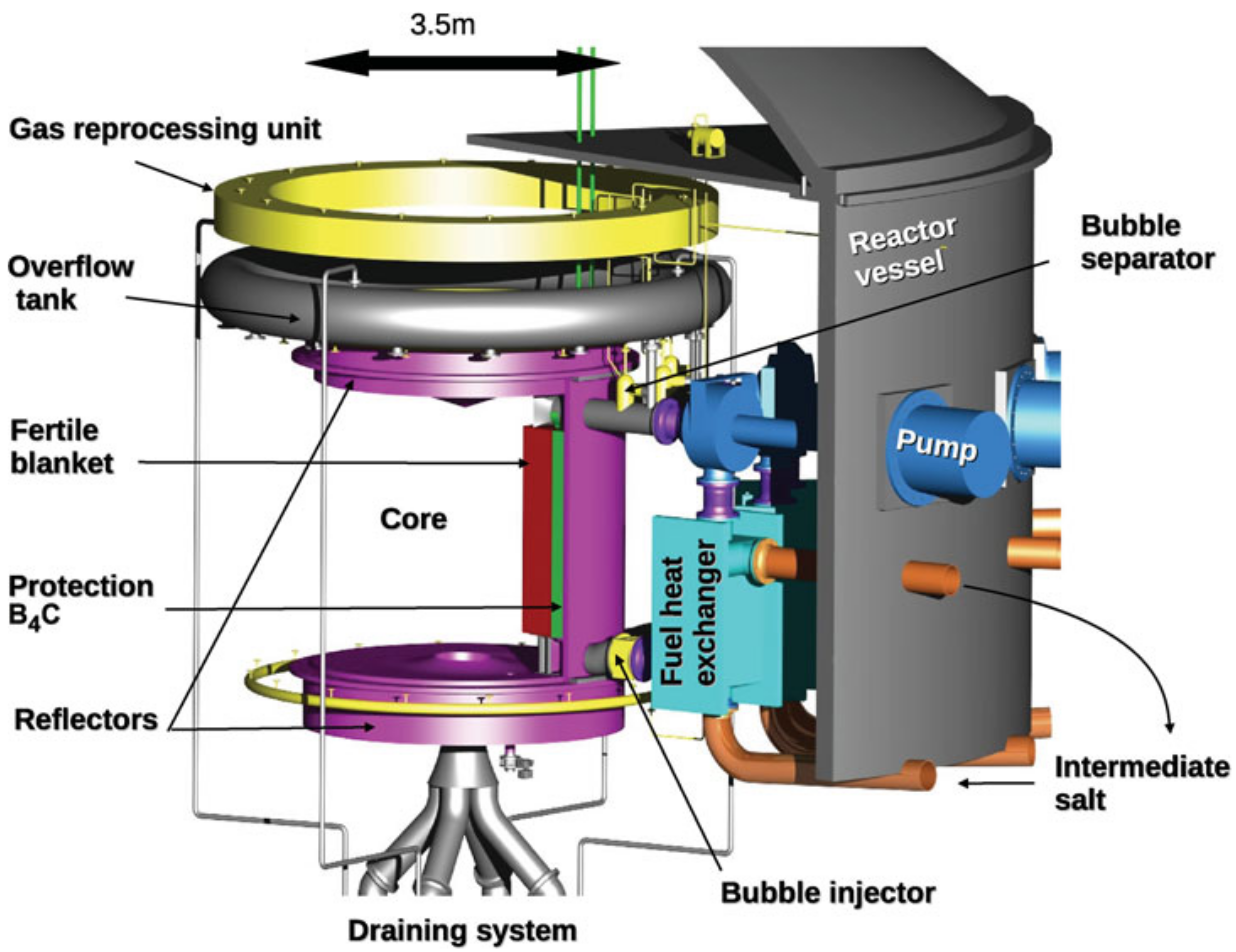
\includegraphics[width=0.8\textwidth]{MSFR}
	\caption{Schematic view of the MSFR concept. Figure reproduced from
	Brovchenko et al. \cite{brovchenko_design-related_2013}.}
	\label{fig:msfr}
\end{figure}
%
\begin{table}[htb!]
    \small
	\caption{Main specifications of the \gls{MSFR} concept
				\cite{serp_molten_2014}.}
	\centering
	\begin{tabular}{ l r }
		\hline
		Parameter & Value \\
		\hline
		Thermal/Electric output [MW$_{\text{th}}$/MW$_{\text{e}}$] & 3000 /
		1500 
		\\
		Salt volume [m$^3$] & 18 \\
		Salt fraction in core & 0.5 \\
		Number of circulation loops & 16 \\
		Nominal flow rate [kg s$^{-1}$] & 18500  \\
		Nominal circulation time [s] & 4.0 \\
		Inlet/outlet temperature [K] & 923 / 1023 \\
		Blanket volume [m$^3$] & 7.3\\
		\hline
	\end{tabular}
	\label{table:msfr}
\end{table}

In the \gls{MSFR} design, fuel salt flows vertically upward through a 9 m$^3$
central core region. At the top of the core, the flow separates into sixteen
smaller external loops, each of which passes through a heat exchanger before
being pumped back into the bottom of the core. The salt also passes through
the online salt reprocessing and gas sparging systems located along the
external loops. A toroidal blanket tank containing fertile salt for breeding
surrounds the core radially. The top and bottom of the core are enclosed
by nickel alloy reflectors. A layer of boron carbide behind the blanket tanks
protects the peripheral equipment from excessive neutron damage. During severe
accidents when core temperatures rise to dangerous levels, the actively
fan-cooled freeze plug at the bottom of the core melts and drains the fuel
salt into a containment vessel designed to keep the salt subcritical. 

Although the \gls{MSFR} is primarily designed to operate on the thorium fuel
cycle, it supports a range of start-up fuel and feed compositions. This
versatility is particularly important for the first few \glspl{MSFR} to be
deployed due to the lack of $^{233}$U reserves required for the initial core
loading. In general, the fuel and blanket salts are approximately composed of
eutectic mixtures of 77.5\% LiF - 22.5\% AcF$_4$; AcF$_4$ represents
actinide fluorides such as uranium, thorium, plutonium, and other \gls{TRU}
fluorides. For an initial composition consisting of $^{232}$Th and $^{233}$U,
the benchmark value for the amount of $^{233}$U for criticality under
normal operating conditions is 2.5 mol\%. However, a neutronic benchmark
study by Brovchenko et al. \cite{brovchenko_neutronic_2019} shows that
different neutronics software with different nuclear data clearly provide
different $k_{eff}$ estimates even with the same isotopic compositions and
temperature distributions. The individual co-authors adjusted the
ratio of $^{232}$Th to $^{233}$U slightly to achieve exact criticality at a
uniform temperature of 973 K for their own neutronics software
\cite{brovchenko_neutronic_2019}. This thesis
performs the same exercise to adjust the inlet and outlet temperatures to
match nominal values.

The thermal and electric power output of the \gls{MSFR} are 3000 MW
$_{\text{th}}$ and 1500 MW$_{\text{e}}$, respectively. The high thermal
efficiency ($\eta_{th}=0.5$) is due to the high operating
temperature. The inlet and outlet temperature
specifications of the fuel salt are 923 K and 1023 K, respectively, for a
minimum 50 K temperature buffer between the
operating temperatures and the melting point of the salt (873 K)
\cite{euratom_final_2015}. The \gls{MSFR} has
heat exchangers and an intermediate coolant loop to isolate the power
conversion system from the highly radioactive fuel salt. This also serves as
a layer of containment between the radioactive material and the outside
environment. The exact composition of the intermediate coolant is not
finalized yet but potential candidates include NaF-NaBF$_4$, FLiNaK,
LiF-ZrF$_4$, and FliBe \cite{merle_concept_2017}.

\subsection{Model Reactor Geometry}

This present work uses the same 2-D square-cylindrical \gls{MSFR} design to
benchmark our results against results published by Fiorina et al.
\cite{fiorina_modelling_2014}. The design is a 2-D axisymmetric representation
of the \gls{MSFR} with the sixteen individual external loops homogenized into
a single outer loop as shown in Figure \ref{fig:msfrgeom}. For the multigroup
group constants calculations in Serpent, the 2-D axisymmetric model is
extended into a 3-D model by a 360-degrees rotation about the
central axis. The material definitions are the same as those specified in the
reference \gls{MSFR} model. Accordingly, the pump and heat exchanger regions
are assumed to be composed of 100\% fuel salt. While this may not be entirely
accurate, the exact details of the pump and heat exchanger systems are still
under active study, and this external loop region is presumed to be of little
neutronic importance due to its position behind the strong boron carbide
neutron absorber layer.
%
\begin{figure}[t!] 
	\centering
	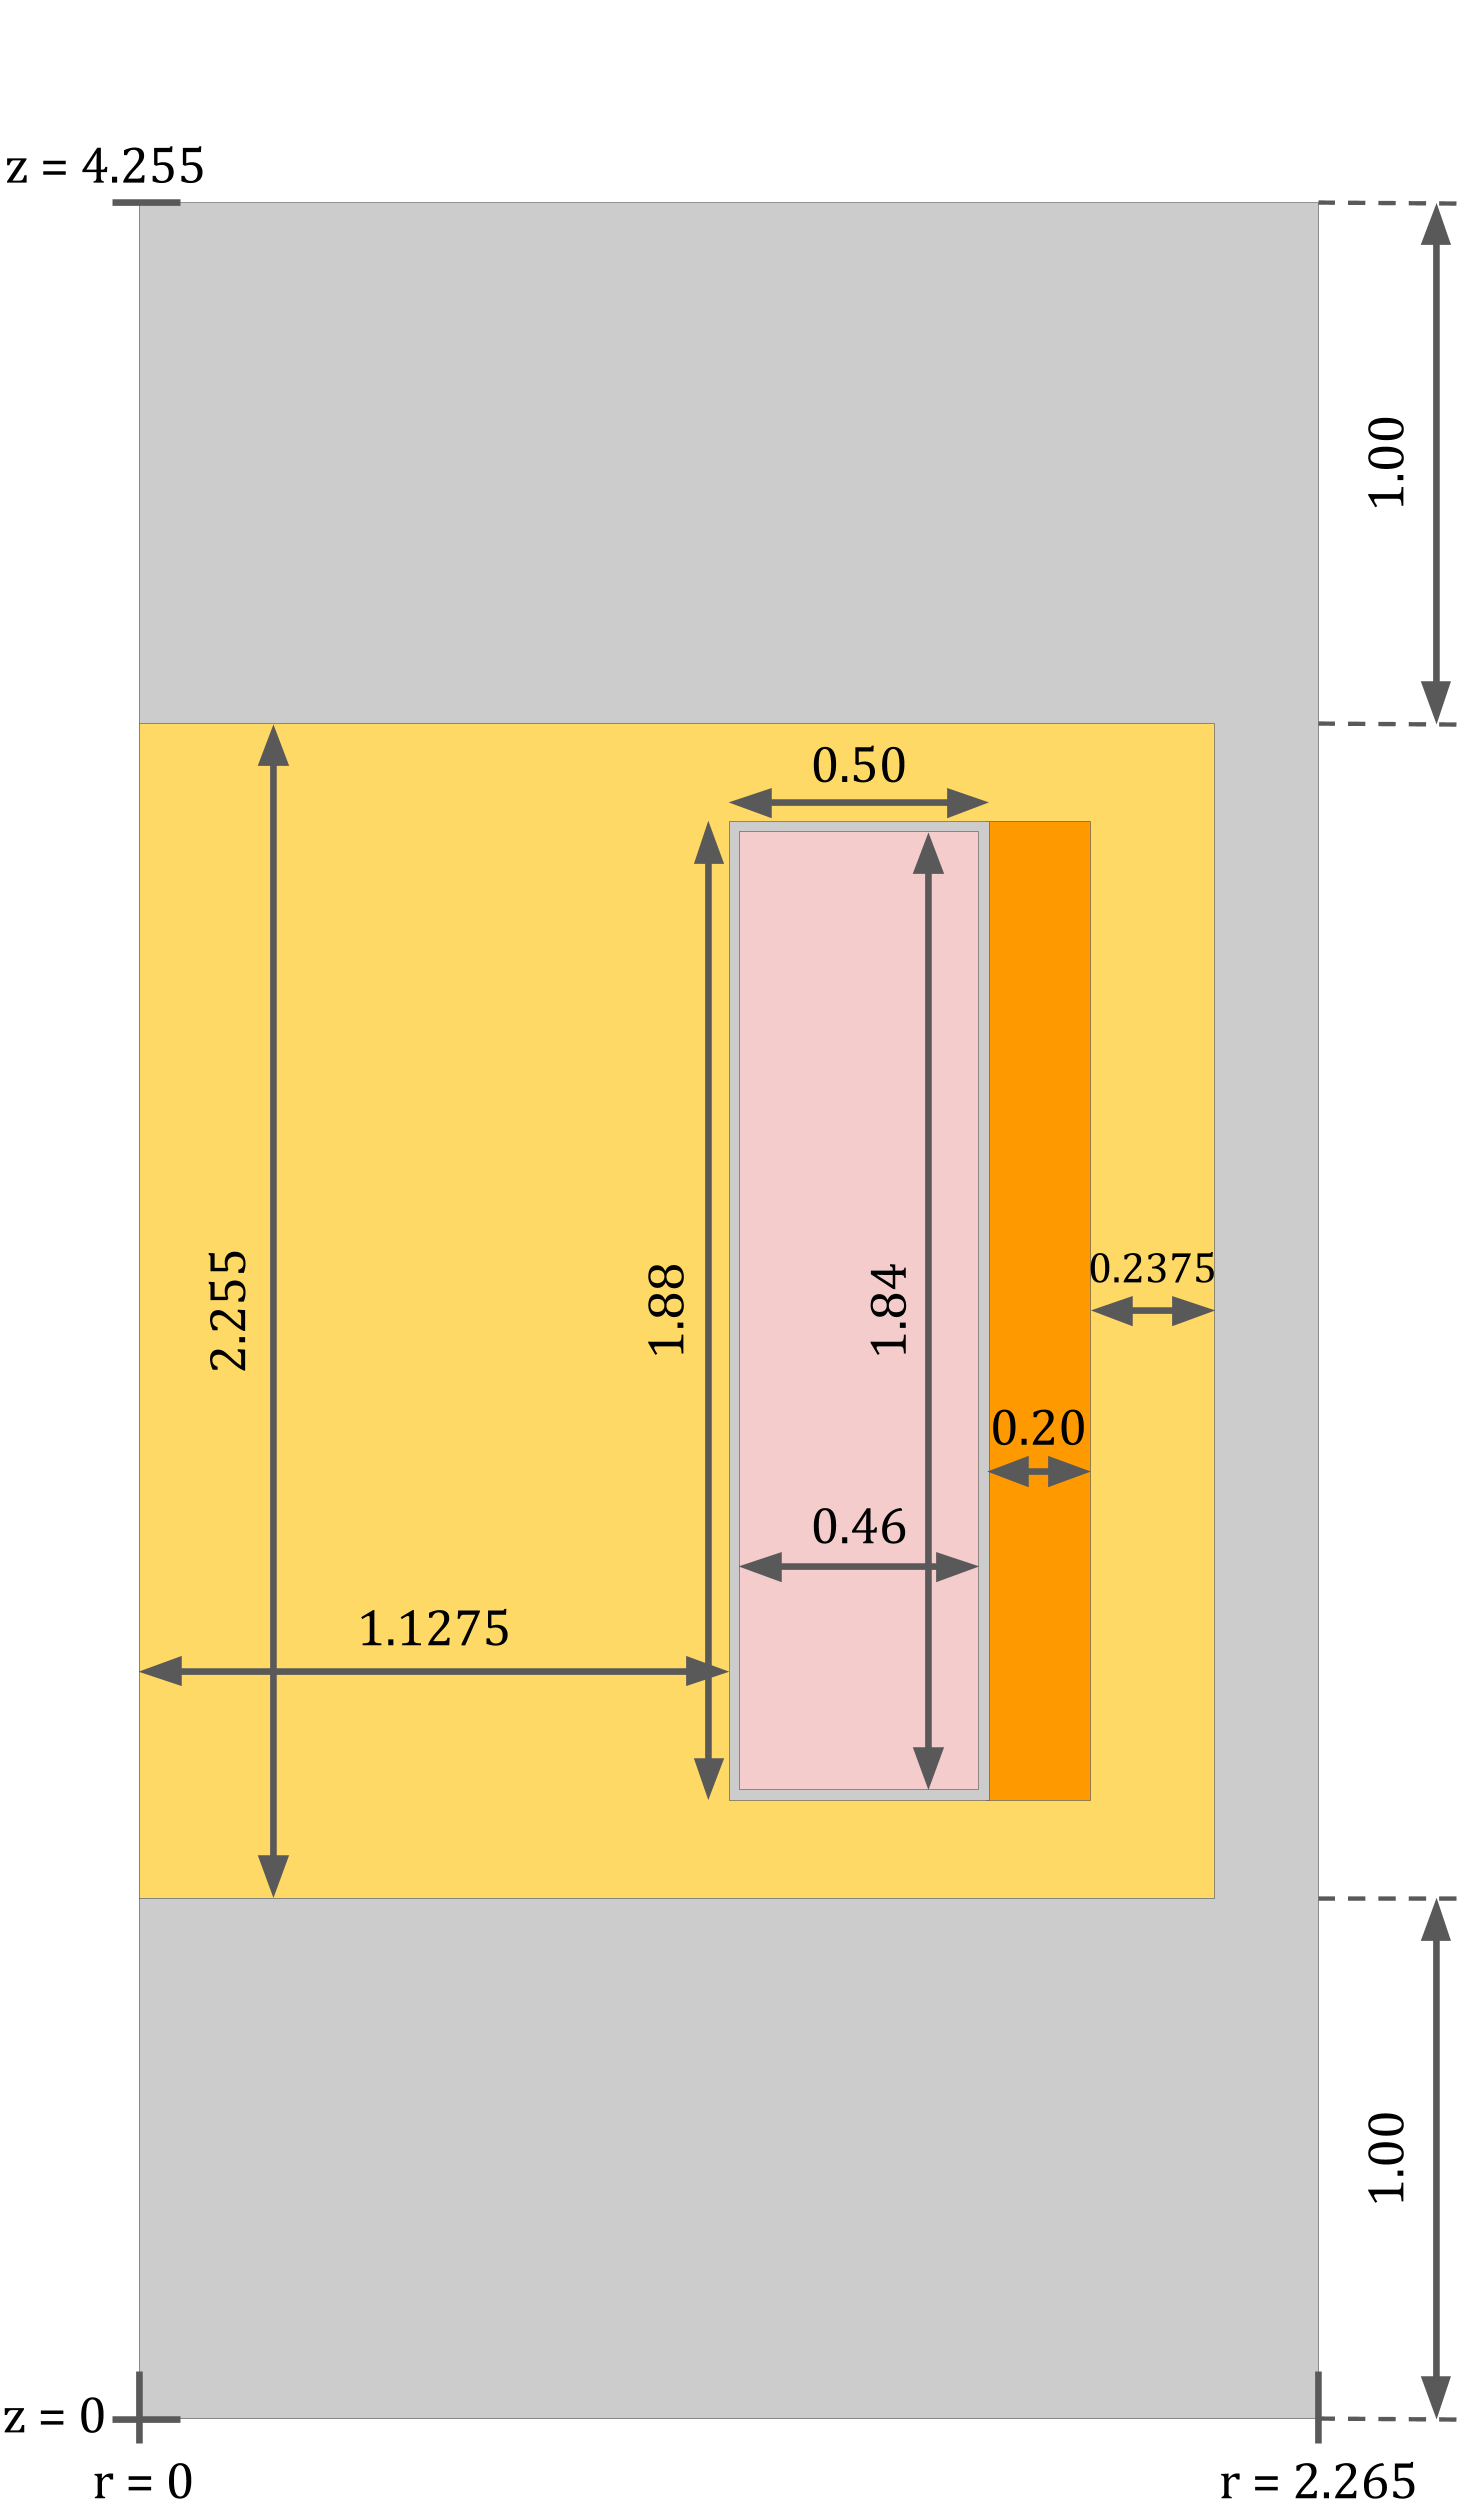
\includegraphics[width=0.5\textwidth]{msfr-geom}
	\caption{2-D axisymmetric model of the \gls{MSFR} core used for the
	simulations in Serpent. All dimensions are in meters.
	\cite{brovchenko_neutronic_2019}}
	\label{fig:msfrgeom}
\end{figure}

Although this present work uses the same 2-D axisymmetric geometry for
generating
group constant data from Serpent, there are two minor differences between the
\gls{MSFR} geometry used in the Moltres model, and the Polimi and TUDelft
models \cite{fiorina_modelling_2014}. Firstly, the reactor geometry for
Moltres excludes the 2-cm-thick structural material around the blanket tank
that separates the fuel and blanket salts. The thickness is much smaller than
the rest of the regions in the geometry and caused issues for meshing. The
neutronics results in Chapter \ref{chap:nts} shows that the overall $k_{eff}$
and other parameters from Moltres show good agreement with that from Serpent.
It also has no direct impact on the temperature distribution results because
this present work solves for the temperature distribution in the primary loop
with homogeneous Neumann boundary conditions on the fuel salt-to-wall
interface. This approach is for consistency with the Polimi and TUDelft
models.

The second difference pertains to the out-of-core section of the primary loop.
The focus for Moltres development has been on core multiphysics over detailed
out-of-core multiphysics. The Moltres model simulates the outer loop as a 1-D
pipe with a pointwise heat sink to represent the heat exchanger. To simulate
the pumps, a Dirichlet boundary condition for velocity at the inlet boundaries
drives the flow in the central core region of the primary loop. At every
timestep, Moltres converges the core and outer loop calculations using Picard
iterations. This approach shares some similarities with the
geometric multiscale modeling approach by Zanetti et al.
\cite{zanetti_geometric_2015}. Future models could create a better
representation of the primary loop by implementing a whole continuous loop
with pressure increases and drops corresponding to the pumps and heat
exchangers.

\subsection{Material Specifications}

This section details the material specifications of the various reactor
components in the \gls{MSFR}.

\subsubsection{Molten Salt}

The reference start-up salt composition for the fuel and blanket salts is
77.5\% LiF - 22.5\% AcF$_4$ (actinide fluorides)
\cite{merle-lucotte_launching_2011}. Typically, researchers working with the
\gls{MSFR}
model tweak the exact actinide composition by varying the $^{232}$Th to
$^{233}$U ratio to obtain a $k_{\text{eff}}$ value of 1 at a uniform
temperature of 973 K \cite{brovchenko_neutronic_2019}. Thus, the exact
actinide compositions vary depending on
the nuclear data library and neutron transport code. This present work uses
a fuel salt composition of 77.5\% LiF - 19.913\% ThF$_4$ - 2.587\%
$^{233}$UF$_4$ for all calculations, which is a simplifying assumption but a
fuel burnup analysis is complex and out of scope for this thesis. Table
\ref{table:prip} shows relevant physical properties of the fuel and blanket
salts.
%
\begin{table}[htb!]
\small
\centering
\caption{Properties of the fuel and blanket salts LiF-AcF$_4$.}
\begin{tabular}{l l r r}
\toprule
Property & Formula & {Value at 973 K} & Validity Range\\
\midrule
Melting temperature [K] & 841 & {N/A} & 1 bar \\
Boiling temperature [K] & 1874 & {N/A} & 1 bar \\
Density, $\rho$ [kg m$^{-3}$] & $4094-0.882 \cdot (T-1008)$ & $4125$ & 893-1123 K \\
Dynamic viscosity, $\mu$ [Pa s] & $\rho \cdot 5.55 \times 10^{-8} \cdot e^{3689/T}$ & $1.015$ & 898-1121 K \\
Thermal conductivity, $k$ [W m$^{-1}$ K$^{-1}$] & $0.928+8.397 \times 10^{-5} \cdot T$ & $0.01010$ & 891-1020 K \\
Specific heat, $c_p$ [J kg$^{-1}$ K$^{-1}$] & $-1111+2.78\cdot T$ & $1594$ & 867-907 K \\
\bottomrule
\end{tabular}
\label{table:prip}
\end{table}

\subsubsection{Structural Materials}

The reflectors on the periphery of the reactor core and the blanket tank are
made of a NiCrW Hastelloy (metal alloy) \cite{brovchenko_neutronic_2019}.
Table \ref{table:refl} details the elemental composition
of the Hastelloy. The alloy has a density
of 10 g$\cdot$cm$^{-3}$. The \gls{MSFR} also includes a 20 cm
layer of boron carbide (B$_4$C) to protect the heat exchangers and pumps from
neutron irradiation. The reference specifications indicate that natural boron
is used, which is composed of 19.8 \% $^{10}$B and 80.2 \% $^{11}$B, with an
overall density of 2.52 g$\cdot$cm$^{-3}$. 
%
\begin{table}[htb!]
\footnotesize
\centering
\caption{Composition (mol \%) of the NiCrW Hastelloy.}
\begin{tabular}{l l l l l l l l l l l l l}
\toprule
Ni & W & Cr & Mo & Fe & Ti & C & Mn & Si & Al & B & P & S \\
\midrule
79.432 & 9.976 & 8.014 & 0.736 & 0.632 & 0.295 & 0.294 & 0.257 & 0.252 & 0.052 & 0.033 & 0.023 & 0.004 \\
\bottomrule
\end{tabular}
\label{table:refl}
\end{table}
